\documentclass[12pt,a4paper]{article}
\usepackage[utf8]{vietnam}
\usepackage{amsmath,amssymb}
\usepackage{tabularx}
\usepackage{tikz}
\usepackage{xcolor}
\usepackage[top=0.6cm, bottom=0.6cm, left=0.6cm, right=0.6cm]{geometry}
\usepackage[dethi]{ex_test}

\SAOPTN{widthSA=2.6,heightSA=0.62}
\setlength{\parskip}{0pt}

% Dong ke cham mo chuan viet tay
\newcommand{\dongke}[1]{%
  \begingroup%
  \setlength{\parskip}{0pt}%
  \baselineskip=18.5pt%
  \vspace{1.0mm}%
  \foreach \i in {1,...,#1}{%
    \noindent{\color{gray!60}\dotfill}\par%
  }%
  \vspace{0.6mm}%
  \endgroup%
}

% Khu vuc bai lam chia 2 cot co vach ngan mo o giua
\newcommand{\dongkeHaiCot}[1]{%
  \par\vspace{0.5mm}%
  \noindent%
  \begin{minipage}[t]{0.485\linewidth}%
    \dongke{#1}%
  \end{minipage}%
  \hfill%
  {\color{gray!60}\vrule}%
  \hfill%
  \begin{minipage}[t]{0.485\linewidth}%
    \dongke{#1}%
  \end{minipage}%
}

% Dinh nghia o bai tap tu luan trong bang
\newcommand{\oBaiTap}[3][5]{%
  \vspace{1.0mm}%
  \noindent\textbf{#2} #3\par%
  \dongke{#1}%
}

\begin{document}
\pagestyle{empty}
% =============================================================================
% ========================= TOAN 8 TUAN 10 BUOI 01 - MA DE 101 =================
% ========================= TRANG 1/2 ==========================================
% =============================================================================
\noindent
\begin{tabularx}{\linewidth}{|X|c|}
\hline
\textbf{PHIẾU KIỂM TRA ĐỊNH KỲ TOÁN 8 - TUẦN 10 - BUỔI 1} & \textbf{Mã đề: 101 - Trang 1/2} \\
\hline
\end{tabularx}

\vspace{1.2mm}

\noindent
\begin{tabularx}{\linewidth}{|p{3.2cm}|X|}
\hline
\centering\textbf{ĐIỂM SỐ} & \centering\textbf{LỜI NHẬN XÉT CỦA THẦY CÔ} \tabularnewline
\hline
\rule{0pt}{1.8cm} & \tabularnewline
\hline
\end{tabularx}

\vspace{1.4mm}
\noindent\textbf{Câu 1 (0,25 điểm).} Tỉ số của hai đoạn thẳng $AB = 6\text{ cm}$ và $CD = 15\text{ cm}$ bằng: \shortans{\frac{2}{5}}\par\vspace{2.0mm}
\noindent\textbf{Câu 2 (0,25 điểm).} Biết $\dfrac{AB}{CD} = \dfrac{A'B'}{C'D'}$ với $AB = 4, CD = 6, A'B' = 6\text{ cm}$. Độ dài $C'D'$ là: \shortans{9\text{ cm}}\par\vspace{2.0mm}
\noindent\textbf{Câu 3 (0,25 điểm).} $\Delta ABC, MN \parallel BC$. Biết $AM = 3, MB = 6, AN = 4\text{ cm}$. Độ dài $NC$ là: \shortans{8\text{ cm}}\par\vspace{2.0mm}
\noindent\textbf{Câu 4 (0,25 điểm).} Bậc của đơn thức $M = -5x^3 y^2 z^4$ là: \shortans{9}\par\vspace{2.0mm}
\noindent\textbf{Câu 5 (0,25 điểm).} Giá trị của $A = 2x^2 y - 3xy$ tại $x = 1, y = -2$ bằng: \shortans{2}\par\vspace{2.0mm}
\noindent\textbf{Câu 6 (0,25 điểm).} Khai triển $(x + 4)^2 = x^2 + ax + 16$. Hệ số $a$ bằng: \shortans{8}\par\vspace{2.0mm}
\noindent\textbf{Câu 7 (0,25 điểm).} Tính nhanh giá trị biểu thức $85^2 - 15^2 = $ \shortans{7\,000}\par\vspace{2.0mm}
\noindent\textbf{Câu 8 (0,25 điểm).} Kết quả phép chia $(15x^3 y^2 - 10x^2 y) : (5x^2 y)$ là: \shortans{3xy - 2}\par\vspace{2.0mm}
\noindent\textbf{Câu 9 (0,25 điểm).} Hình thang cân $ABCD$ ($AB \parallel CD$) có $\widehat{C} = 65^\circ$. Số đo góc $A$ là: \shortans{115^\circ}\par\vspace{2.0mm}
\noindent\textbf{Câu 10 (0,25 điểm).} Cọc cao $1{,}5\text{ m}$ có bóng $2\text{ m}$; bóng cột cờ dài $8\text{ m}$. Cột cờ cao: \shortans{6\text{ m}}\par\vspace{2.0mm}
\vspace{0.2mm}
\noindent\textbf{Câu 11 (3,0 điểm). Thực hiện phép tính (rút gọn nếu có thể):}
\vspace{0.8mm}

\noindent
\begin{tabularx}{\linewidth}{|X|X|}
\hline
\oBaiTap[5]{a) (0,5 điểm)}{$2x(3x^2 - 4x + 1)$} & 
\oBaiTap[5]{b) (0,5 điểm)}{$(x - 2)(x + 3) - x^2$} \\
\hline
\oBaiTap[5]{c) (0,5 điểm)}{$(x + 3)^2 - (x - 3)^2$} & 
\oBaiTap[5]{d) (0,5 điểm)}{$(15x^3 y^2 - 9x^2 y^3 + 6x^2 y^2) : (3x^2 y^2)$} \\
\hline
\oBaiTap[5]{e) (0,5 điểm)}{$(2x + 1)^2 - 4x(x + 1)$} & 
\oBaiTap[5]{f) (0,5 điểm)}{Cho $A = x^3 - 3x^2 + 3x - 1$. Tính giá trị của $A$ tại $x = 101$} \\
\hline
\end{tabularx}

\newpage
% =============================================================================
% ========================= TOAN 8 TUAN 10 BUOI 01 - MA DE 101 =================
% ========================= TRANG 2/2 ==========================================
% =============================================================================
\noindent
\begin{tabularx}{\linewidth}{|X|c|}
\hline
\textbf{TOÁN 8 - TUẦN 10 - BUỔI 1} & \textbf{Mã đề: 101 - Trang 2/2} \\
\hline
\end{tabularx}

\vspace{1.4mm}

\noindent\textbf{Câu 12 (2,0 điểm). Tìm số thực $x$, biết:}
\vspace{0.8mm}

\noindent
\begin{tabularx}{\linewidth}{|X|X|}
\hline
\oBaiTap[5]{a) (0,5 điểm)}{$2x(x - 3) - 2x^2 = 12$} & 
\oBaiTap[5]{b) (0,5 điểm)}{$x(x - 5) + 3(x - 5) = 0$} \\
\hline
\oBaiTap[5]{c) (0,5 điểm)}{$(x + 2)^2 - 9 = 0$} & 
\oBaiTap[5]{d) (0,5 điểm)}{$(2x - 1)^2 = 25$} \\
\hline
\end{tabularx}

\vspace{1.4mm}

\noindent
\begin{tabularx}{\linewidth}{|X|}
\hline
\vspace{0.5mm}
\begin{minipage}[t]{0.64\linewidth}
\vspace{0pt}
\textbf{Câu 13 (2,0 điểm).} Cho tam giác $ABC$. Trên cạnh $AB$ lấy điểm $D$, trên cạnh $AC$ lấy điểm $E$ sao cho $DE \parallel BC$. Cho biết $AD = 6\text{ cm}, DB = 3\text{ cm}, AE = 8\text{ cm}$.\par\vspace{0.4mm}
\textbf{a)} \textbf{(1,0 điểm)} Tính độ dài các đoạn thẳng $EC$ và $AC$.\par\vspace{0.4mm}
\textbf{b)} \textbf{(1,0 điểm)} Qua $E$ kẻ đường thẳng song song với $AB$ cắt cạnh $BC$ tại $F$. Chứng minh tứ giác $BDEF$ là hình bình hành, từ đó suy ra $BF = DE$.
\end{minipage}\hfill
\begin{minipage}[t]{0.34\linewidth}
\vspace{0pt}\centering
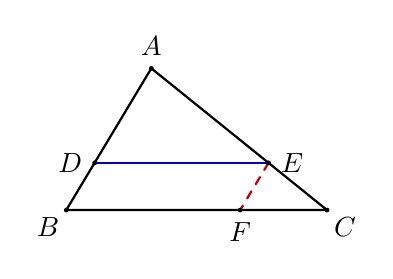
\begin{tikzpicture}[scale=0.72, >=stealth, line join=round, line cap=round]
  \coordinate (B) at (0, 0);
  \coordinate (C) at (4.6, 0);
  \coordinate (A) at (1.5, 2.5);
  \coordinate (D) at (0.5, 0.833);
  \coordinate (E) at (3.567, 0.833);
  \coordinate (F) at (3.067, 0);
  \draw[thick] (A) -- (B) -- (C) -- cycle;
  \draw[thick, blue!85!black] (D) -- (E);
  \draw[thick, red!75!black, dashed] (E) -- (F);
  \fill (A) circle (1.2pt) node[above=1pt] {$A$};
  \fill (B) circle (1.2pt) node[below left=-1pt] {$B$};
  \fill (C) circle (1.2pt) node[below right=-1pt] {$C$};
  \fill (D) circle (1.2pt) node[left=1pt] {$D$};
  \fill (E) circle (1.2pt) node[right=1pt] {$E$};
  \fill (F) circle (1.2pt) node[below=1pt] {$F$};
\end{tikzpicture}
\end{minipage}\par
\vspace{0.4mm}
\noindent\textit{Bài giải:}\dongkeHaiCot{11}
\\ \hline
\end{tabularx}

\vspace{1.4mm}

\noindent
\begin{tabularx}{\linewidth}{|X|}
\hline
\vspace{0.5mm}
\textbf{Câu 14 (0,5 điểm).} Tìm giá trị nhỏ nhất của biểu thức $A = x^2 - 8x + 2045$.\par
\vspace{0.4mm}
\noindent\textit{Bài giải:}\dongkeHaiCot{7}
\\ \hline
\end{tabularx}

\newpage
% =============================================================================
% ========================= TOAN 8 TUAN 10 BUOI 01 - MA DE 102 =================
% ========================= TRANG 1/2 ==========================================
% =============================================================================
\noindent
\begin{tabularx}{\linewidth}{|X|c|}
\hline
\textbf{PHIẾU KIỂM TRA ĐỊNH KỲ TOÁN 8 - TUẦN 10 - BUỔI 1} & \textbf{Mã đề: 102 - Trang 1/2} \\
\hline
\end{tabularx}

\vspace{1.2mm}

\noindent
\begin{tabularx}{\linewidth}{|p{3.2cm}|X|}
\hline
\centering\textbf{ĐIỂM SỐ} & \centering\textbf{LỜI NHẬN XÉT CỦA THẦY CÔ} \tabularnewline
\hline
\rule{0pt}{1.8cm} & \tabularnewline
\hline
\end{tabularx}

\vspace{1.4mm}
\noindent\textbf{Câu 1 (0,25 điểm).} Tỉ số của hai đoạn thẳng $AB = 8\text{ cm}$ và $CD = 20\text{ cm}$ bằng: \shortans{\frac{2}{5}}\par\vspace{2.0mm}
\noindent\textbf{Câu 2 (0,25 điểm).} Biết $\dfrac{AB}{CD} = \dfrac{A'B'}{C'D'}$ với $AB = 6, CD = 9, A'B' = 8\text{ cm}$. Độ dài $C'D'$ là: \shortans{12\text{ cm}}\par\vspace{2.0mm}
\noindent\textbf{Câu 3 (0,25 điểm).} $\Delta ABC, MN \parallel BC$. Biết $AM = 2, MB = 4, AN = 5\text{ cm}$. Độ dài $NC$ là: \shortans{10\text{ cm}}\par\vspace{2.0mm}
\noindent\textbf{Câu 4 (0,25 điểm).} Bậc của đơn thức $N = 7x^4 y^3 z^2$ là: \shortans{9}\par\vspace{2.0mm}
\noindent\textbf{Câu 5 (0,25 điểm).} Giá trị của $B = 3x^2 y - 4xy$ tại $x = 1, y = -2$ bằng: \shortans{2}\par\vspace{2.0mm}
\noindent\textbf{Câu 6 (0,25 điểm).} Khai triển $(x - 5)^2 = x^2 - bx + 25$. Hệ số $b$ bằng: \shortans{10}\par\vspace{2.0mm}
\noindent\textbf{Câu 7 (0,25 điểm).} Tính nhanh giá trị biểu thức $75^2 - 25^2 = $ \shortans{5\,000}\par\vspace{2.0mm}
\noindent\textbf{Câu 8 (0,25 điểm).} Kết quả phép chia $(12x^4 y^3 - 8x^3 y^2) : (4x^3 y^2)$ là: \shortans{3xy - 2}\par\vspace{2.0mm}
\noindent\textbf{Câu 9 (0,25 điểm).} Hình thang cân $ABCD$ ($AB \parallel CD$) có $\widehat{D} = 70^\circ$. Số đo góc $B$ là: \shortans{110^\circ}\par\vspace{2.0mm}
\noindent\textbf{Câu 10 (0,25 điểm).} Cọc cao $1{,}2\text{ m}$ có bóng $1{,}5\text{ m}$; bóng cột đèn dài $5\text{ m}$. Cột đèn cao: \shortans{4\text{ m}}\par\vspace{2.0mm}
\vspace{0.2mm}
\noindent\textbf{Câu 11 (3,0 điểm). Thực hiện phép tính (rút gọn nếu có thể):}
\vspace{0.8mm}

\noindent
\begin{tabularx}{\linewidth}{|X|X|}
\hline
\oBaiTap[5]{a) (0,5 điểm)}{$3x(2x^2 - 3x + 2)$} & 
\oBaiTap[5]{b) (0,5 điểm)}{$(x - 3)(x + 4) - x^2$} \\
\hline
\oBaiTap[5]{c) (0,5 điểm)}{$(x + 4)^2 - (x - 4)^2$} & 
\oBaiTap[5]{d) (0,5 điểm)}{$(18x^4 y^2 - 12x^3 y^3 + 6x^3 y^2) : (6x^3 y^2)$} \\
\hline
\oBaiTap[5]{e) (0,5 điểm)}{$(3x + 1)^2 - 6x(x + 1) - 3x^2$} & 
\oBaiTap[5]{f) (0,5 điểm)}{Cho $B = x^3 + 3x^2 + 3x + 1$. Tính giá trị của $B$ tại $x = 99$} \\
\hline
\end{tabularx}

\newpage
% =============================================================================
% ========================= TOAN 8 TUAN 10 BUOI 01 - MA DE 102 =================
% ========================= TRANG 2/2 ==========================================
% =============================================================================
\noindent
\begin{tabularx}{\linewidth}{|X|c|}
\hline
\textbf{TOÁN 8 - TUẦN 10 - BUỔI 1} & \textbf{Mã đề: 102 - Trang 2/2} \\
\hline
\end{tabularx}

\vspace{1.4mm}

\noindent\textbf{Câu 12 (2,0 điểm). Tìm số thực $x$, biết:}
\vspace{0.8mm}

\noindent
\begin{tabularx}{\linewidth}{|X|X|}
\hline
\oBaiTap[5]{a) (0,5 điểm)}{$3x(x - 2) - 3x^2 = 18$} & 
\oBaiTap[5]{b) (0,5 điểm)}{$x(x - 4) + 2(x - 4) = 0$} \\
\hline
\oBaiTap[5]{c) (0,5 điểm)}{$(x + 3)^2 - 16 = 0$} & 
\oBaiTap[5]{d) (0,5 điểm)}{$(2x + 1)^2 = 25$} \\
\hline
\end{tabularx}

\vspace{1.4mm}

\noindent
\begin{tabularx}{\linewidth}{|X|}
\hline
\vspace{0.5mm}
\begin{minipage}[t]{0.64\linewidth}
\vspace{0pt}
\textbf{Câu 13 (2,0 điểm).} Cho tam giác $ABC$. Trên cạnh $AB$ lấy điểm $D$, trên cạnh $AC$ lấy điểm $E$ sao cho $DE \parallel BC$. Cho biết $AD = 8\text{ cm}, DB = 4\text{ cm}, AE = 10\text{ cm}$.\par\vspace{0.4mm}
\textbf{a)} \textbf{(1,0 điểm)} Tính độ dài các đoạn thẳng $EC$ và $AC$.\par\vspace{0.4mm}
\textbf{b)} \textbf{(1,0 điểm)} Qua $E$ kẻ đường thẳng song song với $AB$ cắt cạnh $BC$ tại $F$. Chứng minh tứ giác $BDEF$ là hình bình hành, từ đó suy ra $BF = DE$.
\end{minipage}\hfill
\begin{minipage}[t]{0.34\linewidth}
\vspace{0pt}\centering
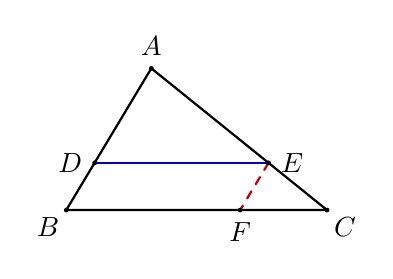
\begin{tikzpicture}[scale=0.72, >=stealth, line join=round, line cap=round]
  \coordinate (B) at (0, 0);
  \coordinate (C) at (4.6, 0);
  \coordinate (A) at (1.5, 2.5);
  \coordinate (D) at (0.5, 0.833);
  \coordinate (E) at (3.567, 0.833);
  \coordinate (F) at (3.067, 0);
  \draw[thick] (A) -- (B) -- (C) -- cycle;
  \draw[thick, blue!85!black] (D) -- (E);
  \draw[thick, red!75!black, dashed] (E) -- (F);
  \fill (A) circle (1.2pt) node[above=1pt] {$A$};
  \fill (B) circle (1.2pt) node[below left=-1pt] {$B$};
  \fill (C) circle (1.2pt) node[below right=-1pt] {$C$};
  \fill (D) circle (1.2pt) node[left=1pt] {$D$};
  \fill (E) circle (1.2pt) node[right=1pt] {$E$};
  \fill (F) circle (1.2pt) node[below=1pt] {$F$};
\end{tikzpicture}
\end{minipage}\par
\vspace{0.4mm}
\noindent\textit{Bài giải:}\dongkeHaiCot{11}
\\ \hline
\end{tabularx}

\vspace{1.4mm}

\noindent
\begin{tabularx}{\linewidth}{|X|}
\hline
\vspace{0.5mm}
\textbf{Câu 14 (0,5 điểm).} Tìm giá trị nhỏ nhất của biểu thức $B = x^2 - 10x + 2051$.\par
\vspace{0.4mm}
\noindent\textit{Bài giải:}\dongkeHaiCot{7}
\\ \hline
\end{tabularx}

\newpage
% =============================================================================
% ========================= TOAN 8 TUAN 10 BUOI 01 - MA DE 103 =================
% ========================= TRANG 1/2 ==========================================
% =============================================================================
\noindent
\begin{tabularx}{\linewidth}{|X|c|}
\hline
\textbf{PHIẾU KIỂM TRA ĐỊNH KỲ TOÁN 8 - TUẦN 10 - BUỔI 1} & \textbf{Mã đề: 103 - Trang 1/2} \\
\hline
\end{tabularx}

\vspace{1.2mm}

\noindent
\begin{tabularx}{\linewidth}{|p{3.2cm}|X|}
\hline
\centering\textbf{ĐIỂM SỐ} & \centering\textbf{LỜI NHẬN XÉT CỦA THẦY CÔ} \tabularnewline
\hline
\rule{0pt}{1.8cm} & \tabularnewline
\hline
\end{tabularx}

\vspace{1.4mm}
\noindent\textbf{Câu 1 (0,25 điểm).} Tỉ số của hai đoạn thẳng $AB = 9\text{ cm}$ và $CD = 21\text{ cm}$ bằng: \shortans{\frac{3}{7}}\par\vspace{2.0mm}
\noindent\textbf{Câu 2 (0,25 điểm).} Biết $\dfrac{AB}{CD} = \dfrac{A'B'}{C'D'}$ với $AB = 5, CD = 10, A'B' = 7\text{ cm}$. Độ dài $C'D'$ là: \shortans{14\text{ cm}}\par\vspace{2.0mm}
\noindent\textbf{Câu 3 (0,25 điểm).} $\Delta ABC, MN \parallel BC$. Biết $AM = 4, MB = 8, AN = 3\text{ cm}$. Độ dài $NC$ là: \shortans{6\text{ cm}}\par\vspace{2.0mm}
\noindent\textbf{Câu 4 (0,25 điểm).} Bậc của đơn thức $P = -3x^2 y^4 z^3$ là: \shortans{9}\par\vspace{2.0mm}
\noindent\textbf{Câu 5 (0,25 điểm).} Giá trị của $C = 2x^2 y - 5xy$ tại $x = 1, y = -2$ bằng: \shortans{6}\par\vspace{2.0mm}
\noindent\textbf{Câu 6 (0,25 điểm).} Khai triển $(2x + 3)^2 = 4x^2 + cx + 9$. Hệ số $c$ bằng: \shortans{12}\par\vspace{2.0mm}
\noindent\textbf{Câu 7 (0,25 điểm).} Tính nhanh giá trị biểu thức $65^2 - 35^2 = $ \shortans{3\,000}\par\vspace{2.0mm}
\noindent\textbf{Câu 8 (0,25 điểm).} Kết quả phép chia $(18x^3 y^3 - 12x^2 y^2) : (6x^2 y^2)$ là: \shortans{3xy - 2}\par\vspace{2.0mm}
\noindent\textbf{Câu 9 (0,25 điểm).} Hình thang cân $ABCD$ ($AB \parallel CD$) có $\widehat{C} = 75^\circ$. Số đo góc $A$ là: \shortans{105^\circ}\par\vspace{2.0mm}
\noindent\textbf{Câu 10 (0,25 điểm).} Cọc cao $2\text{ m}$ có bóng $3\text{ m}$; bóng cây xanh dài $9\text{ m}$. Cây xanh cao: \shortans{6\text{ m}}\par\vspace{2.0mm}
\vspace{0.2mm}
\noindent\textbf{Câu 11 (3,0 điểm). Thực hiện phép tính (rút gọn nếu có thể):}
\vspace{0.8mm}

\noindent
\begin{tabularx}{\linewidth}{|X|X|}
\hline
\oBaiTap[5]{a) (0,5 điểm)}{$4x(2x^2 - x + 3)$} & 
\oBaiTap[5]{b) (0,5 điểm)}{$(x - 4)(x + 5) - x^2$} \\
\hline
\oBaiTap[5]{c) (0,5 điểm)}{$(x + 5)^2 - (x - 5)^2$} & 
\oBaiTap[5]{d) (0,5 điểm)}{$(20x^3 y^3 - 15x^2 y^4 + 10x^2 y^3) : (5x^2 y^3)$} \\
\hline
\oBaiTap[5]{e) (0,5 điểm)}{$(2x - 1)^2 - 4x(x - 1)$} & 
\oBaiTap[5]{f) (0,5 điểm)}{Cho $C = x^3 - 6x^2 + 12x - 8$. Tính giá trị của $C$ tại $x = 102$} \\
\hline
\end{tabularx}

\newpage
% =============================================================================
% ========================= TOAN 8 TUAN 10 BUOI 01 - MA DE 103 =================
% ========================= TRANG 2/2 ==========================================
% =============================================================================
\noindent
\begin{tabularx}{\linewidth}{|X|c|}
\hline
\textbf{TOÁN 8 - TUẦN 10 - BUỔI 1} & \textbf{Mã đề: 103 - Trang 2/2} \\
\hline
\end{tabularx}

\vspace{1.4mm}

\noindent\textbf{Câu 12 (2,0 điểm). Tìm số thực $x$, biết:}
\vspace{0.8mm}

\noindent
\begin{tabularx}{\linewidth}{|X|X|}
\hline
\oBaiTap[5]{a) (0,5 điểm)}{$4x(x - 2) - 4x^2 = 16$} & 
\oBaiTap[5]{b) (0,5 điểm)}{$x(x - 6) + 4(x - 6) = 0$} \\
\hline
\oBaiTap[5]{c) (0,5 điểm)}{$(x + 1)^2 - 25 = 0$} & 
\oBaiTap[5]{d) (0,5 điểm)}{$(3x - 1)^2 = 16$} \\
\hline
\end{tabularx}

\vspace{1.4mm}

\noindent
\begin{tabularx}{\linewidth}{|X|}
\hline
\vspace{0.5mm}
\begin{minipage}[t]{0.64\linewidth}
\vspace{0pt}
\textbf{Câu 13 (2,0 điểm).} Cho tam giác $ABC$. Trên cạnh $AB$ lấy điểm $D$, trên cạnh $AC$ lấy điểm $E$ sao cho $DE \parallel BC$. Cho biết $AD = 9\text{ cm}, DB = 3\text{ cm}, AE = 12\text{ cm}$.\par\vspace{0.4mm}
\textbf{a)} \textbf{(1,0 điểm)} Tính độ dài các đoạn thẳng $EC$ và $AC$.\par\vspace{0.4mm}
\textbf{b)} \textbf{(1,0 điểm)} Qua $E$ kẻ đường thẳng song song với $AB$ cắt cạnh $BC$ tại $F$. Chứng minh tứ giác $BDEF$ là hình bình hành, từ đó suy ra $BF = DE$.
\end{minipage}\hfill
\begin{minipage}[t]{0.34\linewidth}
\vspace{0pt}\centering
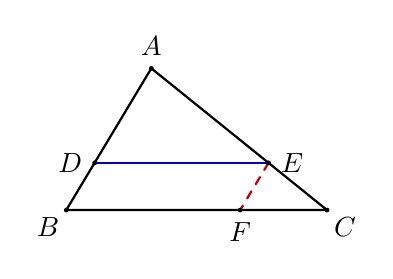
\begin{tikzpicture}[scale=0.72, >=stealth, line join=round, line cap=round]
  \coordinate (B) at (0, 0);
  \coordinate (C) at (4.6, 0);
  \coordinate (A) at (1.5, 2.5);
  \coordinate (D) at (0.5, 0.833);
  \coordinate (E) at (3.567, 0.833);
  \coordinate (F) at (3.067, 0);
  \draw[thick] (A) -- (B) -- (C) -- cycle;
  \draw[thick, blue!85!black] (D) -- (E);
  \draw[thick, red!75!black, dashed] (E) -- (F);
  \fill (A) circle (1.2pt) node[above=1pt] {$A$};
  \fill (B) circle (1.2pt) node[below left=-1pt] {$B$};
  \fill (C) circle (1.2pt) node[below right=-1pt] {$C$};
  \fill (D) circle (1.2pt) node[left=1pt] {$D$};
  \fill (E) circle (1.2pt) node[right=1pt] {$E$};
  \fill (F) circle (1.2pt) node[below=1pt] {$F$};
\end{tikzpicture}
\end{minipage}\par
\vspace{0.4mm}
\noindent\textit{Bài giải:}\dongkeHaiCot{11}
\\ \hline
\end{tabularx}

\vspace{1.4mm}

\noindent
\begin{tabularx}{\linewidth}{|X|}
\hline
\vspace{0.5mm}
\textbf{Câu 14 (0,5 điểm).} Tìm giá trị nhỏ nhất của biểu thức $C = x^2 - 6x + 2036$.\par
\vspace{0.4mm}
\noindent\textit{Bài giải:}\dongkeHaiCot{7}
\\ \hline
\end{tabularx}

\newpage
% =============================================================================
% ========================= TOAN 8 TUAN 10 BUOI 01 - MA DE 104 =================
% ========================= TRANG 1/2 ==========================================
% =============================================================================
\noindent
\begin{tabularx}{\linewidth}{|X|c|}
\hline
\textbf{PHIẾU KIỂM TRA ĐỊNH KỲ TOÁN 8 - TUẦN 10 - BUỔI 1} & \textbf{Mã đề: 104 - Trang 1/2} \\
\hline
\end{tabularx}

\vspace{1.2mm}

\noindent
\begin{tabularx}{\linewidth}{|p{3.2cm}|X|}
\hline
\centering\textbf{ĐIỂM SỐ} & \centering\textbf{LỜI NHẬN XÉT CỦA THẦY CÔ} \tabularnewline
\hline
\rule{0pt}{1.8cm} & \tabularnewline
\hline
\end{tabularx}

\vspace{1.4mm}
\noindent\textbf{Câu 1 (0,25 điểm).} Tỉ số của hai đoạn thẳng $AB = 12\text{ cm}$ và $CD = 28\text{ cm}$ bằng: \shortans{\frac{3}{7}}\par\vspace{2.0mm}
\noindent\textbf{Câu 2 (0,25 điểm).} Biết $\dfrac{AB}{CD} = \dfrac{A'B'}{C'D'}$ với $AB = 4, CD = 8, A'B' = 9\text{ cm}$. Độ dài $C'D'$ là: \shortans{18\text{ cm}}\par\vspace{2.0mm}
\noindent\textbf{Câu 3 (0,25 điểm).} $\Delta ABC, MN \parallel BC$. Biết $AM = 3, MB = 9, AN = 2\text{ cm}$. Độ dài $NC$ là: \shortans{6\text{ cm}}\par\vspace{2.0mm}
\noindent\textbf{Câu 4 (0,25 điểm).} Bậc của đơn thức $Q = 6x^5 y^2 z^2$ là: \shortans{9}\par\vspace{2.0mm}
\noindent\textbf{Câu 5 (0,25 điểm).} Giá trị của $D = 4x^2 y - 5xy$ tại $x = 1, y = -2$ bằng: \shortans{2}\par\vspace{2.0mm}
\noindent\textbf{Câu 6 (0,25 điểm).} Khai triển $(3x - 2)^2 = 9x^2 - dx + 4$. Hệ số $d$ bằng: \shortans{12}\par\vspace{2.0mm}
\noindent\textbf{Câu 7 (0,25 điểm).} Tính nhanh giá trị biểu thức $95^2 - 5^2 = $ \shortans{9\,000}\par\vspace{2.0mm}
\noindent\textbf{Câu 8 (0,25 điểm).} Kết quả phép chia $(21x^4 y^2 - 14x^3 y) : (7x^3 y)$ là: \shortans{3xy - 2}\par\vspace{2.0mm}
\noindent\textbf{Câu 9 (0,25 điểm).} Hình thang cân $ABCD$ ($AB \parallel CD$) có $\widehat{D} = 80^\circ$. Số đo góc $B$ là: \shortans{100^\circ}\par\vspace{2.0mm}
\noindent\textbf{Câu 10 (0,25 điểm).} Cọc cao $1{,}5\text{ m}$ có bóng $2{,}5\text{ m}$; bóng toà nhà dài $15\text{ m}$. Toà nhà cao: \shortans{9\text{ m}}\par\vspace{2.0mm}
\vspace{0.2mm}
\noindent\textbf{Câu 11 (3,0 điểm). Thực hiện phép tính (rút gọn nếu có thể):}
\vspace{0.8mm}

\noindent
\begin{tabularx}{\linewidth}{|X|X|}
\hline
\oBaiTap[5]{a) (0,5 điểm)}{$5x(2x^2 - 3x + 1)$} & 
\oBaiTap[5]{b) (0,5 điểm)}{$(x - 5)(x + 6) - x^2$} \\
\hline
\oBaiTap[5]{c) (0,5 điểm)}{$(x + 2)^2 - (x - 2)^2$} & 
\oBaiTap[5]{d) (0,5 điểm)}{$(24x^4 y^3 - 16x^3 y^4 + 8x^3 y^3) : (8x^3 y^3)$} \\
\hline
\oBaiTap[5]{e) (0,5 điểm)}{$(3x - 1)^2 - 9x(x - 1) - 3x$} & 
\oBaiTap[5]{f) (0,5 điểm)}{Cho $D = x^3 + 6x^2 + 12x + 8$. Tính giá trị của $D$ tại $x = 98$} \\
\hline
\end{tabularx}

\newpage
% =============================================================================
% ========================= TOAN 8 TUAN 10 BUOI 01 - MA DE 104 =================
% ========================= TRANG 2/2 ==========================================
% =============================================================================
\noindent
\begin{tabularx}{\linewidth}{|X|c|}
\hline
\textbf{TOÁN 8 - TUẦN 10 - BUỔI 1} & \textbf{Mã đề: 104 - Trang 2/2} \\
\hline
\end{tabularx}

\vspace{1.4mm}

\noindent\textbf{Câu 12 (2,0 điểm). Tìm số thực $x$, biết:}
\vspace{0.8mm}

\noindent
\begin{tabularx}{\linewidth}{|X|X|}
\hline
\oBaiTap[5]{a) (0,5 điểm)}{$5x(x - 2) - 5x^2 = 20$} & 
\oBaiTap[5]{b) (0,5 điểm)}{$x(x - 7) + 3(x - 7) = 0$} \\
\hline
\oBaiTap[5]{c) (0,5 điểm)}{$(x + 4)^2 - 9 = 0$} & 
\oBaiTap[5]{d) (0,5 điểm)}{$(3x + 1)^2 = 16$} \\
\hline
\end{tabularx}

\vspace{1.4mm}

\noindent
\begin{tabularx}{\linewidth}{|X|}
\hline
\vspace{0.5mm}
\begin{minipage}[t]{0.64\linewidth}
\vspace{0pt}
\textbf{Câu 13 (2,0 điểm).} Cho tam giác $ABC$. Trên cạnh $AB$ lấy điểm $D$, trên cạnh $AC$ lấy điểm $E$ sao cho $DE \parallel BC$. Cho biết $AD = 10\text{ cm}, DB = 5\text{ cm}, AE = 14\text{ cm}$.\par\vspace{0.4mm}
\textbf{a)} \textbf{(1,0 điểm)} Tính độ dài các đoạn thẳng $EC$ và $AC$.\par\vspace{0.4mm}
\textbf{b)} \textbf{(1,0 điểm)} Qua $E$ kẻ đường thẳng song song với $AB$ cắt cạnh $BC$ tại $F$. Chứng minh tứ giác $BDEF$ là hình bình hành, từ đó suy ra $BF = DE$.
\end{minipage}\hfill
\begin{minipage}[t]{0.34\linewidth}
\vspace{0pt}\centering
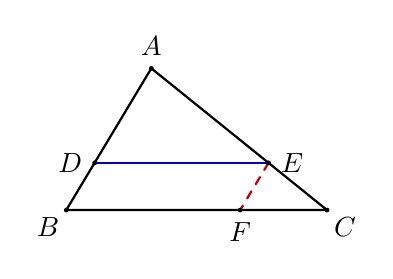
\begin{tikzpicture}[scale=0.72, >=stealth, line join=round, line cap=round]
  \coordinate (B) at (0, 0);
  \coordinate (C) at (4.6, 0);
  \coordinate (A) at (1.5, 2.5);
  \coordinate (D) at (0.5, 0.833);
  \coordinate (E) at (3.567, 0.833);
  \coordinate (F) at (3.067, 0);
  \draw[thick] (A) -- (B) -- (C) -- cycle;
  \draw[thick, blue!85!black] (D) -- (E);
  \draw[thick, red!75!black, dashed] (E) -- (F);
  \fill (A) circle (1.2pt) node[above=1pt] {$A$};
  \fill (B) circle (1.2pt) node[below left=-1pt] {$B$};
  \fill (C) circle (1.2pt) node[below right=-1pt] {$C$};
  \fill (D) circle (1.2pt) node[left=1pt] {$D$};
  \fill (E) circle (1.2pt) node[right=1pt] {$E$};
  \fill (F) circle (1.2pt) node[below=1pt] {$F$};
\end{tikzpicture}
\end{minipage}\par
\vspace{0.4mm}
\noindent\textit{Bài giải:}\dongkeHaiCot{11}
\\ \hline
\end{tabularx}

\vspace{1.4mm}

\noindent
\begin{tabularx}{\linewidth}{|X|}
\hline
\vspace{0.5mm}
\textbf{Câu 14 (0,5 điểm).} Tìm giá trị nhỏ nhất của biểu thức $D = x^2 - 12x + 2064$.\par
\vspace{0.4mm}
\noindent\textit{Bài giải:}\dongkeHaiCot{7}
\\ \hline
\end{tabularx}
\end{document}
